\chapter{Implementación}\label{ch:Implementación}

En este capítulo se describen las principales escenas que componen el simulador, las máquinas de estado que gestionan el flujo de cada una, las acciones que los usuarios pueden realizar, y los scripts más relevantes que soportan la funcionalidad del sistema. El simulador está diseñado para guiar al usuario a través de una experiencia educativa interactiva y estructurada, permitiendo un aprendizaje inmersivo en el contexto de un laboratorio de química inorgánica.

\section{Fases de los Experimentos}
Los experimentos en el simulador están estructurados en cinco fases principales, cada una diseñada para facilitar la comprensión y ejecución de los procesos químicos involucrados. Estas fases aseguran que el usuario avance de manera lógica y progresiva, consolidando conocimientos y habilidades a lo largo de la actividad.

\subsection{Introducción}
En esta fase inicial, se da la bienvenida al usuario con una explicación clara del experimento y sus objetivos principales. Se destaca el contexto químico de la actividad, los materiales necesarios, y una descripción breve pero detallada del fenómeno que se observará. Esta etapa motiva al usuario y establece las bases para comprender los conceptos químicos que serán explorados durante el experimento.
\subsection{Balanceo de Ecuaciones}
El usuario aprende sobre las reacciones químicas involucradas en el experimento a través del análisis y balanceo de ecuaciones. Se le proporciona una ecuación inicial que deberá balancear para garantizar que la cantidad de átomos en ambos lados sea equivalente. El sistema guía al usuario paso a paso, explicando los conceptos básicos y proporciones estequiométricas, mientras utiliza el teclado numérico interactivo para ingresar los coeficientes correctos.
\subsection{Selección y Creación}
El usuario selecciona los elementos necesarios desde la tabla periódica virtual y los combina en el área de creación para formar los compuestos requeridos. A través de gestos intuitivos, como el de pinchar o agarrar, se seleccionan materiales como líquidos o sólidos, que luego se transforman en objetos interactivos listos para el experimento. El sistema proporciona retroalimentación visual para indicar que los compuestos se han preparado correctamente antes de proceder a la experimentación.
\subsection{Experimentación}
En esta etapa, el usuario lleva a cabo el experimento siguiendo instrucciones precisas y detalladas. Se realizan acciones como agregar líquidos o sólidos a recipientes, encender un mechero, calentar materiales, o combinar reactivos, observando los cambios físicos y químicos en tiempo real. Cada acción está respaldada por efectos visuales y sonoros que simulan fenómenos como la liberación de gases, formación de humo, cambios de color y producción de calor o luz, creando una experiencia inmersiva y educativa.
\subsection{Explicación}
Finalmente, el usuario recibe una explicación detallada de los resultados obtenidos durante el experimento. Esta fase resalta los principios químicos involucrados, como reacciones redox, formación de compuestos o cambios energéticos. Se utilizan gráficos y representaciones visuales para reforzar el aprendizaje, asegurando que el usuario comprenda plenamente el fenómeno observado y su relevancia en el contexto de la química.
\newpage
\section{Escenas Principales}
\subsection{Hub}
En la escena del Hub, se implementó una máquina de estados finita (FSM) para gestionar las transiciones entre las diferentes opciones disponibles, como el acceso al tutorial o a los experimentos. Este diseño permite una navegación fluida y estructurada, asegurando que el usuario pueda seleccionar y avanzar hacia las actividades deseadas de manera eficiente.

\begin{figure}[thbp]
    \centering
    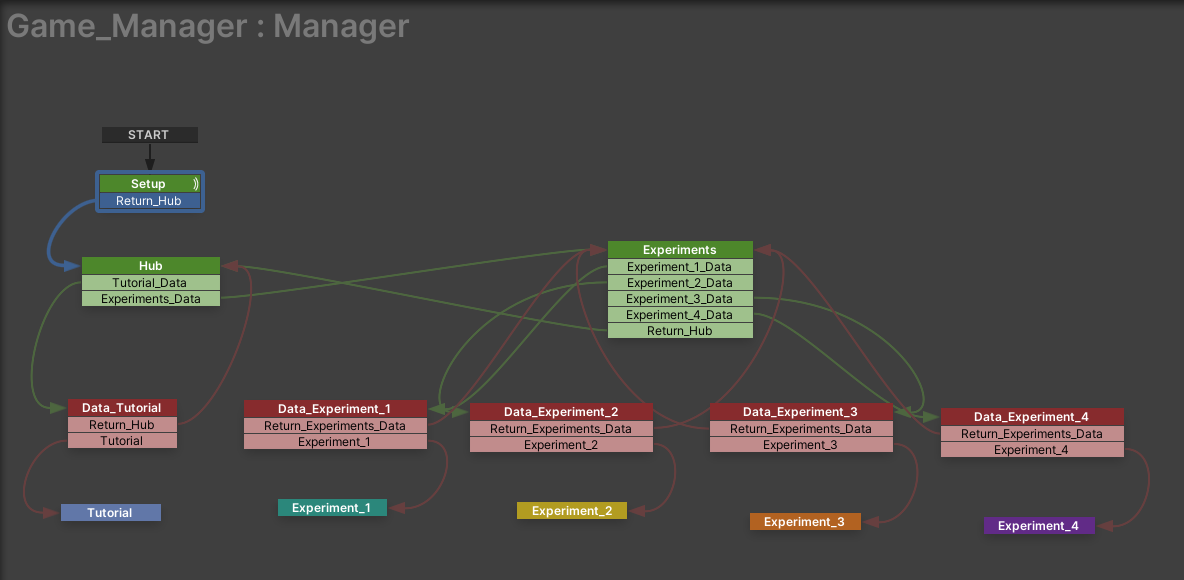
\includegraphics[width=0.7\textwidth, height = 7cm]{img/chapter05/Hub.png}
    \caption{Flujo de la escena Hub}
    \label{fig:FSM_Hub}
\end{figure}

Para implementar y manejar esta máquina de estados, se utilizó el script \texttt{MenuController}, que se encuentra detallado en la (\autoref{script:MenuController}). Este script es responsable de la lógica principal, como el manejo de eventos, la actualización de datos en la interfaz y la ejecución de las transiciones correspondientes dentro del flujo definido por la FSM.
La \autoref{fig:FSM_Hub} muestra el diagrama de la máquina de estados que estructura esta escena.

\subsection{Tutorial}
La escena de Tutorial utiliza una FSM para organizar las etapas de aprendizaje, desde la introducción hasta la realización de interacciones clave. Esta máquina guía al usuario a través de un proceso secuencial diseñado para familiarizarlo con las mecánicas del simulador y las herramientas virtuales.
\begin{figure}[thbp]
    \centering
    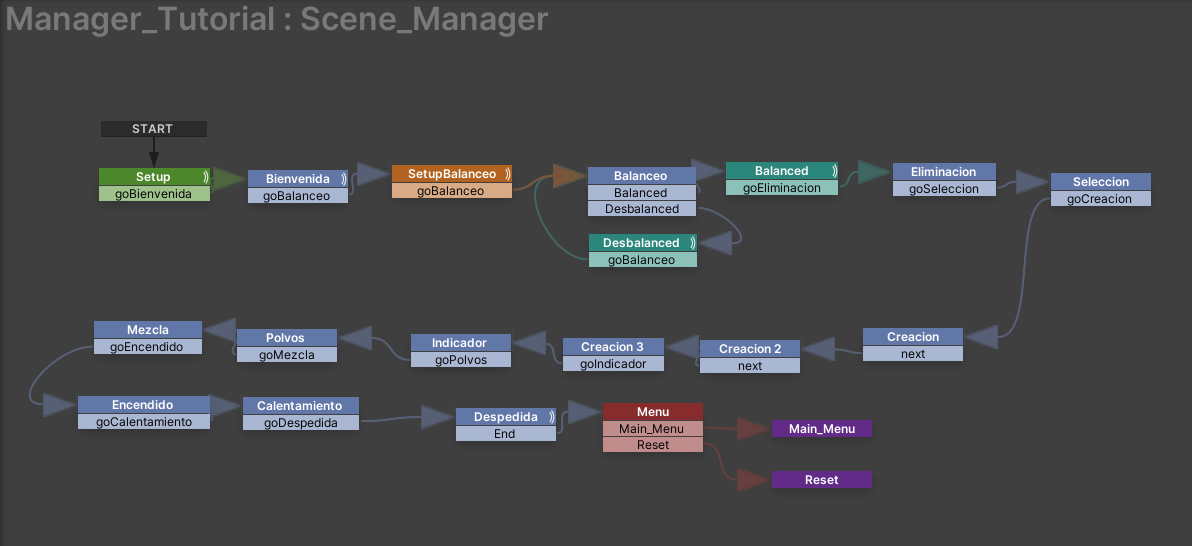
\includegraphics[width=0.7\textwidth, height = 7cm]{img/chapter05/Tutorial.png}
    \caption{Flujo de la escena Tutorial}
    \label{fig:FSM_Tutorial}
\end{figure}

La escena comienza con una bienvenida que introduce al usuario a las herramientas y conceptos básicos del simulador. Luego, se presentan tareas prácticas que incluyen el balanceo de ecuaciones, la selección y mezcla de sustancias, y el encendido y calentamiento de materiales, todo respaldado por retroalimentación visual y auditiva. Finalmente, la escena concluye con una despedida que refuerza los conceptos aprendidos y permite al usuario volver al menú principal.
\newpage
\subsection{Experimento 1}
La escena del Experimento 1 está diseñada para gestionar tareas específicas relacionadas con el balanceo de ecuaciones químicas y la manipulación de sustancias. La FSM controla cada etapa del experimento, permitiendo avanzar solo cuando las condiciones necesarias se cumplen.
\begin{figure}[thbp]
    \centering
    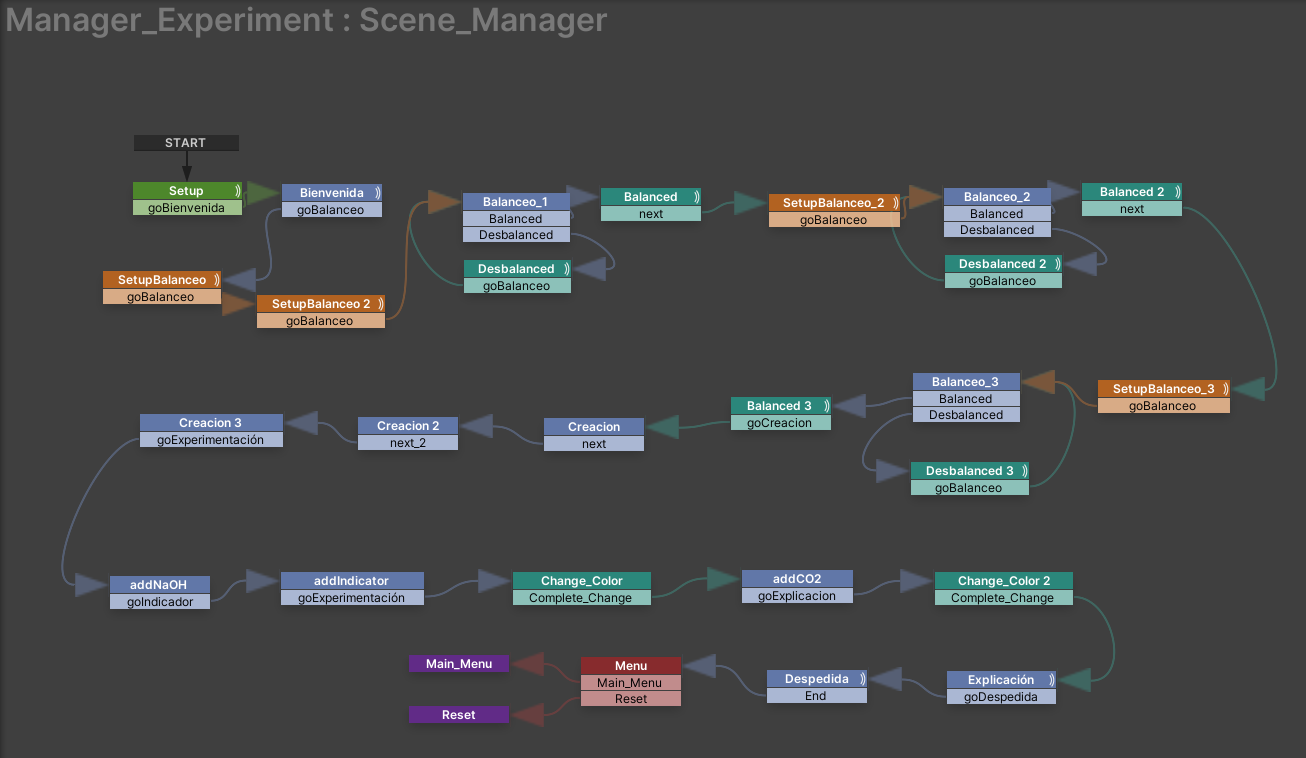
\includegraphics[width=0.7\textwidth, height = 7cm]{img/chapter05/Experimento_01.png}
    \caption{Flujo de la escena Experimento 1}
    \label{fig:FSM_E1}
\end{figure}

El flujo del experimento incluye pasos como el balanceo de ecuaciones químicas, la selección de sustancias específicas y su combinación, y la observación de cambios visuales en los materiales. Cada etapa está respaldada por retroalimentación visual y auditiva para mejorar la comprensión del usuario. Además, se utilizan efectos visuales, como cambios de color, para simular reacciones químicas.

El script \texttt{Experiment\_1\_Manager}, documentado en la \autoref{script:Experiment1Manager} valida las acciones del usuario, como la correcta combinación de sustancias, y activa eventos en la FSM para reflejar el progreso en tiempo real. Además, se manejan efectos visuales para representar las reacciones químicas de forma precisa. La estructura del flujo de esta escena se puede observar en la \autoref{fig:FSM_E1}.

\subsection{Experimento 2}
En el Experimento 2, la FSM organiza actividades que involucran la validación de mezclas químicas y la manipulación de temperatura. Los estados aseguran que las condiciones del experimento, como el tiempo de calentamiento o las combinaciones correctas, se cumplan antes de proceder.
\begin{figure}[thbp]
    \centering
    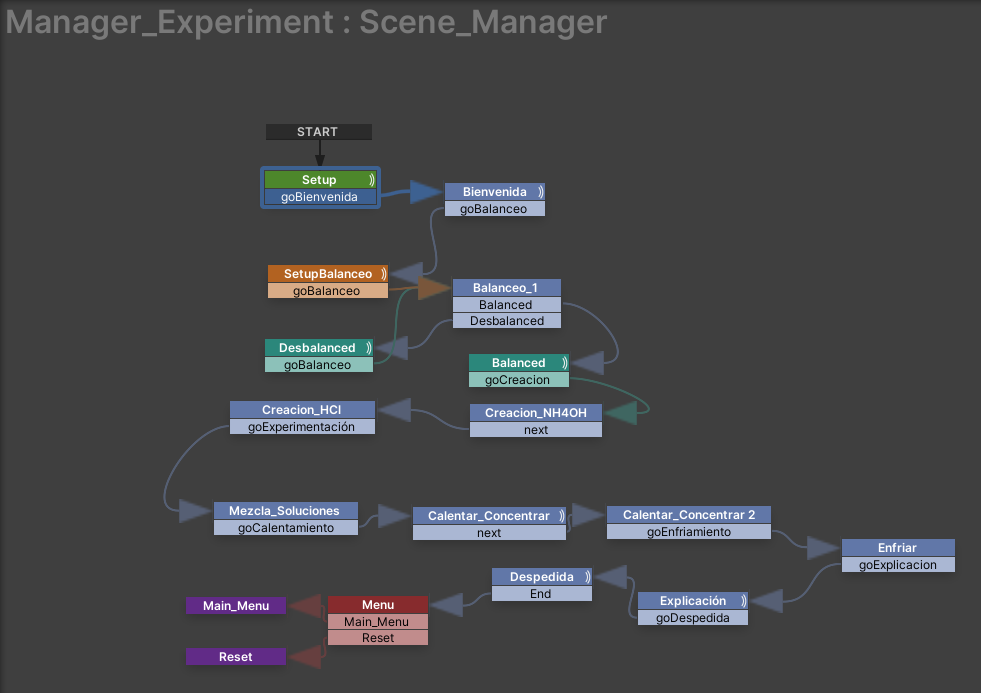
\includegraphics[width=0.7\textwidth, height = 7cm]{img/chapter05/Experimento_02.png}
    \caption{Flujo de la escena Experimento 2}
    \label{fig:FSM_E2}
\end{figure}

El script \texttt{Experiment\_2\_Manager}, documentado en la \autoref{script:Experiment2Manager}, implementa la lógica para monitorear estos parámetros y activar transiciones en la FSM, además de generar efectos visuales y auditivos que simulan las reacciones químicas.

\subsection{Experimento 3}
La FSM del Experimento 3 gestiona las combinaciones de sustancias y la activación de reacciones exotérmicas, estructurando el flujo del experimento para garantizar que cada acción del usuario sea validada antes de avanzar.
\begin{figure}[thbp]
    \centering
    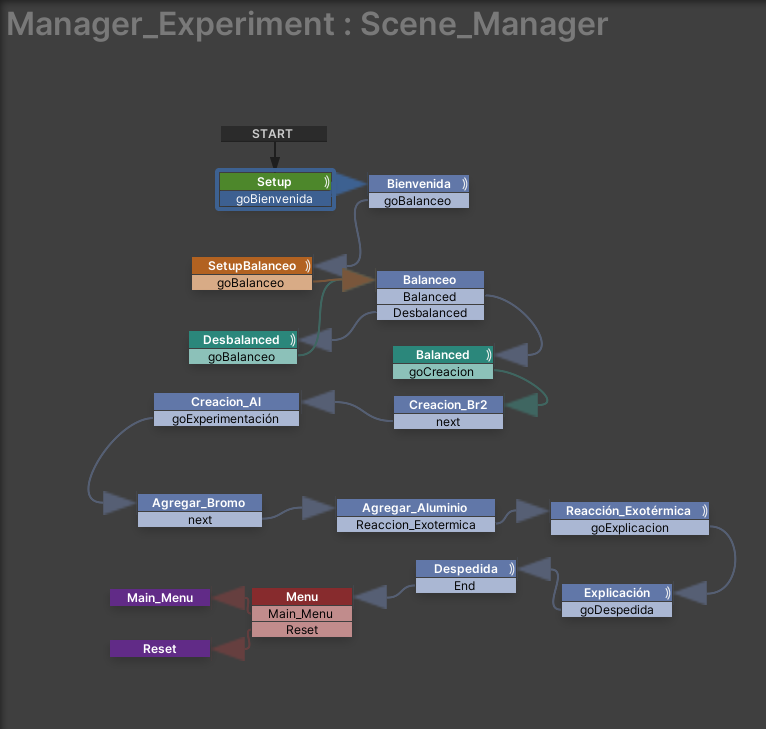
\includegraphics[width=0.7\textwidth, height = 7cm]{img/chapter05/Experimento_03.png}
    \caption{Flujo de la escena Experimento 3}
    \label{fig:FSM_E3}
\end{figure}

El script \texttt{Experiment\_3\_Manager}, documentado en la \autoref{script:Experiment3Manager}, se encarga de verificar las combinaciones realizadas y de controlar eventos visuales, como el llenado de recipientes, ofreciendo una experiencia interactiva y alineada con los objetivos del experimento.

\subsection{Experimento 4}
El Experimento 4 utiliza una FSM para gestionar tareas relacionadas con la manipulación de magnesio y dióxido de carbono sólido (hielo seco). Las etapas incluyen la preparación inicial, el encendido del magnesio, y la observación de una reacción exotérmica que genera luz intensa y subproductos químicos.
\begin{figure}[thbp]
    \centering
    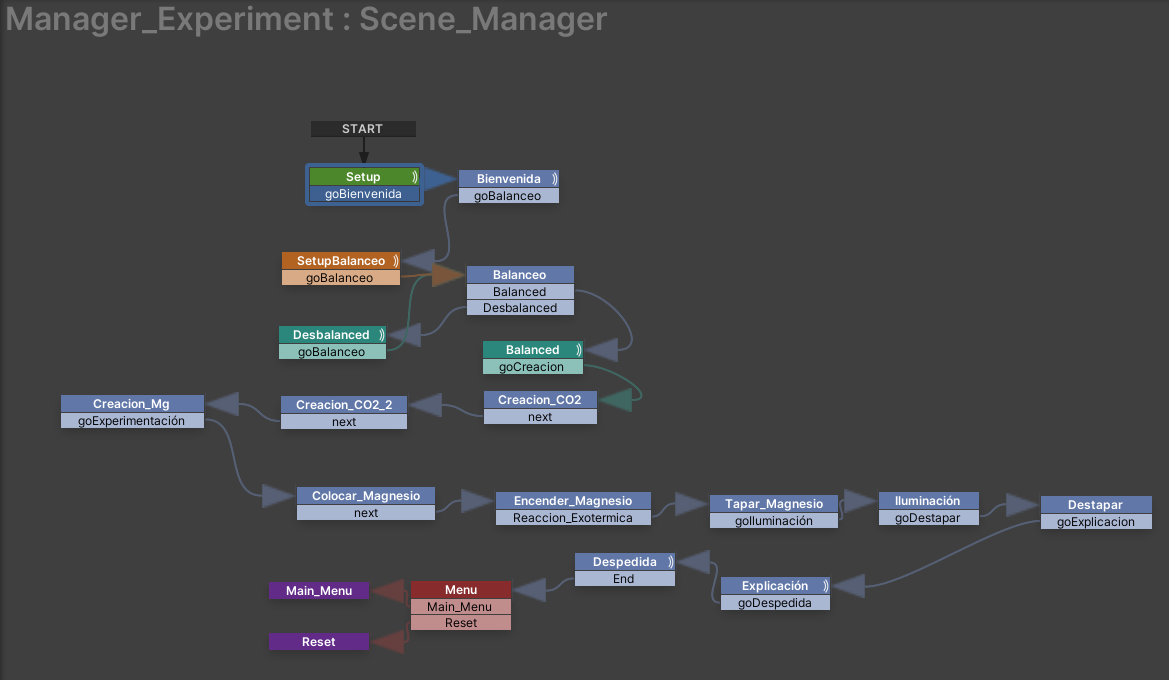
\includegraphics[width=0.7\textwidth, height = 7cm]{img/chapter05/Experimento_04.png}
    \caption{Flujo de la escena Experimento 4}
    \label{fig:FSM_E4}
\end{figure}

El script \texttt{Experiment\_4\_Manager}, documentado en la \autoref{script:Experiment4Manager},  valida las acciones del usuario, como la correcta combinación de sustancias, y coordina eventos visuales y auditivos que simulan los procesos químicos involucrados. Este enfoque asegura que la experiencia sea inmersiva y técnicamente precisa.
\newpage
\section{Acciones del Usuario}
En el simulador, los usuarios tienen la capacidad de interactuar con diversos elementos y realizar acciones que son esenciales para completar los experimentos. Estas interacciones están diseñadas para ser intuitivas y están respaldadas por un sistema de lógica basado en máquinas de estados y scripts específicos que controlan los flujos de acción. A continuación, se describen las principales acciones disponibles.
\subsection{Manipulación de Objetos}
El usuario puede tomar objetos interactuables, como recipientes, herramientas de laboratorio y materiales, utilizando los gestos configurados con el SDK de Oculus. 
\begin{figure}[thbp]
    \centering
    \begin{subfigure}[b]{0.4\linewidth}
        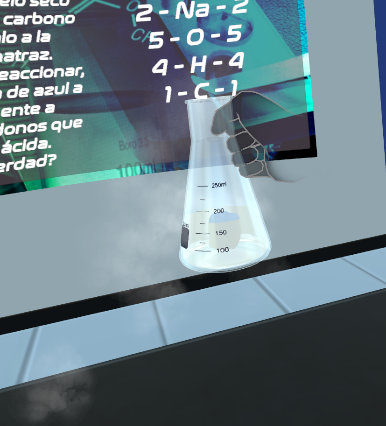
\includegraphics[width=\linewidth, height = 5cm]{img/chapter05/Manipulación_01.png}
    \end{subfigure}
    \begin{subfigure}[b]{0.4\linewidth}
        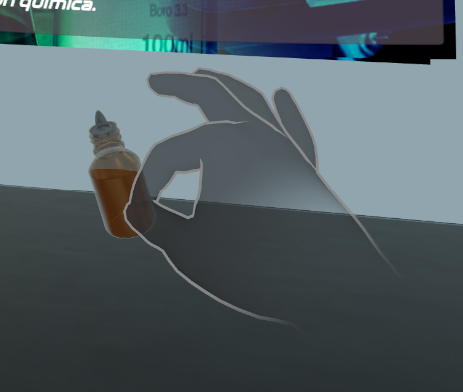
\includegraphics[width=\linewidth, height = 5cm]{img/chapter05/Pinch (2).png}
    \end{subfigure}
    \begin{subfigure}[b]{0.4\linewidth}
        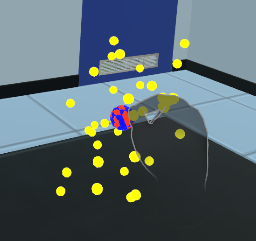
\includegraphics[width=\linewidth, height = 5cm]{img/chapter05/Agarre.png}
    \end{subfigure}
    \caption{Diversas Interacciones con objetos}
\end{figure}
\newpage
\subsection{Selección de Elementos en la Tabla Periódica}
El simulador incluye una tabla periódica interactiva donde el usuario puede seleccionar elementos químicos con un gesto de toque directo. Los elementos seleccionados se transforman en sus representaciones virtuales (modelos atómicos o sustancias químicas) y pueden ser llevados al área de creación o al experimento.
\begin{figure}[thbp]
    \centering
    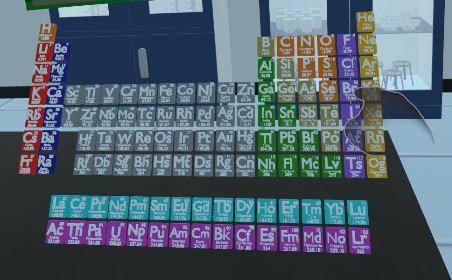
\includegraphics[width=0.6\textwidth, height = 5cm]{img/chapter05/Tabla_Periodica.png}
    \caption{Tabla Periódica}
    \label{fig:Tabla_Periódica}
\end{figure}
\subsection{Creación y Manipulación de Compuestos}
Los compuestos químicos se generan combinando elementos o materiales en áreas específicas designadas. El sistema valida automáticamente las combinaciones correctas y actualiza el estado de los experimentos, proporcionando retroalimentación visual y textual sobre el progreso.
\begin{figure}[thbp]
    \centering
    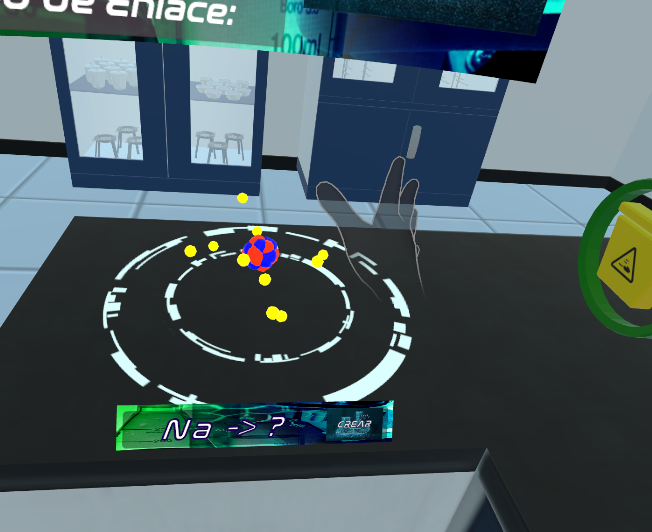
\includegraphics[width=0.7\textwidth, height = 7cm]{img/chapter05/Zona_Creación (2).png}
    \caption{Zona de Creación de compuestos}
    \label{fig:Creación_Compuestos}
\end{figure}
\newpage
\subsection{Encendido de Mecheros y Materiales}
El encendido se realiza al acercar la flama del encendedor al mechero o a algún compuesto que deba quemarse. Una vez que el encendedor está lo suficientemente cerca, el sistema detecta la proximidad y activa la acción correspondiente, generando los efectos visuales y sonoros que simulan la ignición.
\begin{figure}[thbp]
    \centering
    \begin{subfigure}[b]{0.3\linewidth}
        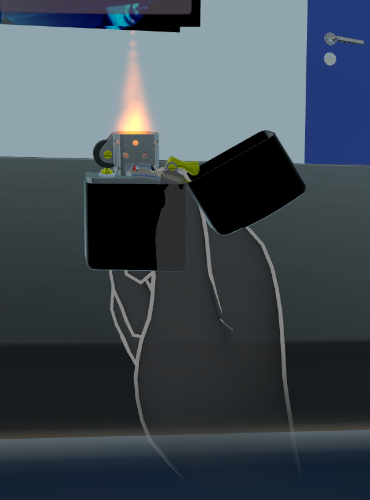
\includegraphics[width=\linewidth, height = 5cm]{img/chapter05/Encendido01.png}
        \caption{Uso de encendedor}
        \label{fig:Encendedor}
    \end{subfigure}
    \begin{subfigure}[b]{0.3\linewidth}
        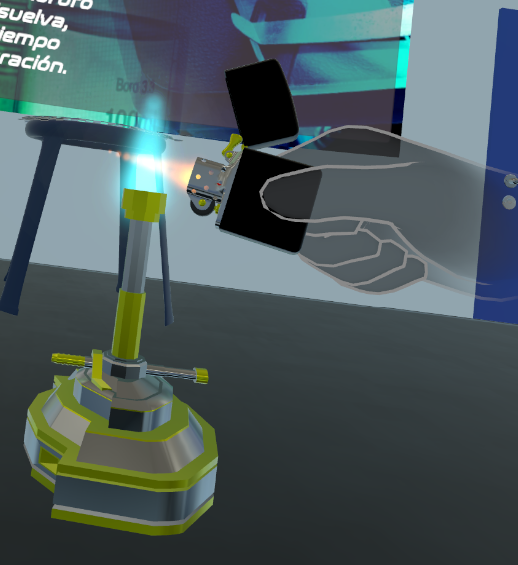
\includegraphics[width=\linewidth, height = 5cm]{img/chapter05/Encendido02.png}
        \caption{Encendido de mechero}
        \label{fig:Mechero}
    \end{subfigure}
    \begin{subfigure}[b]{0.3\linewidth}
        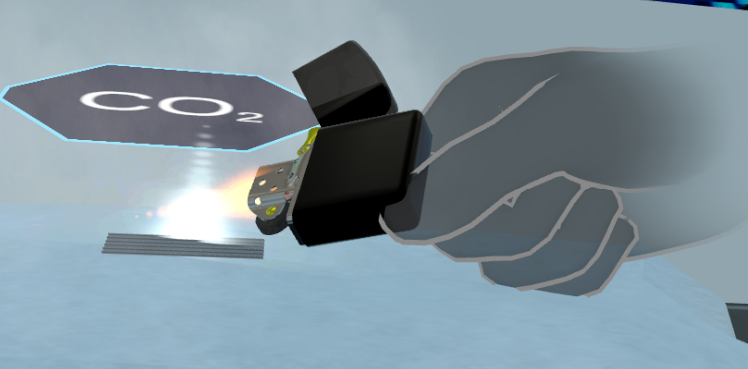
\includegraphics[width=\linewidth, height = 5cm]{img/chapter05/Encendido03.png}
        \caption{Encendidos de material}
        \label{fig:Material_Encendido}
    \end{subfigure}
    \caption{Encendido diverso}
\end{figure}
\subsection{Eliminación de Elementos}
Para eliminar un elemento seleccionado, el usuario debe llevarlo a la zona de desecho. Una vez en esta área, el sistema lo detecta y elimina automáticamente, permitiendo mantener un espacio de trabajo ordenado y sin materiales innecesarios.
\begin{figure}[thbp]
    \centering
    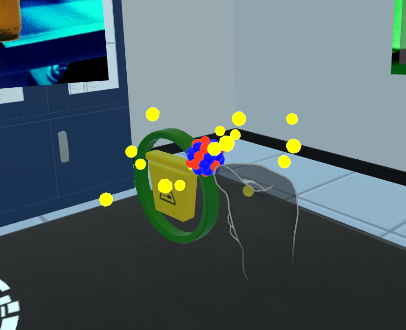
\includegraphics[width=0.7\textwidth, height = 7cm]{img/chapter05/Eliminación.png}
    \caption{Eliminación de un elemento}
    \label{fig:Eliminación}
\end{figure}
\newpage
\subsection{Acciones Relacionadas con Líquidos}
Las interacciones con líquidos están diseñadas para ser inmersivas y detalladas, permitiendo al usuario:
\begin{figure}[thbp]
    \centering
    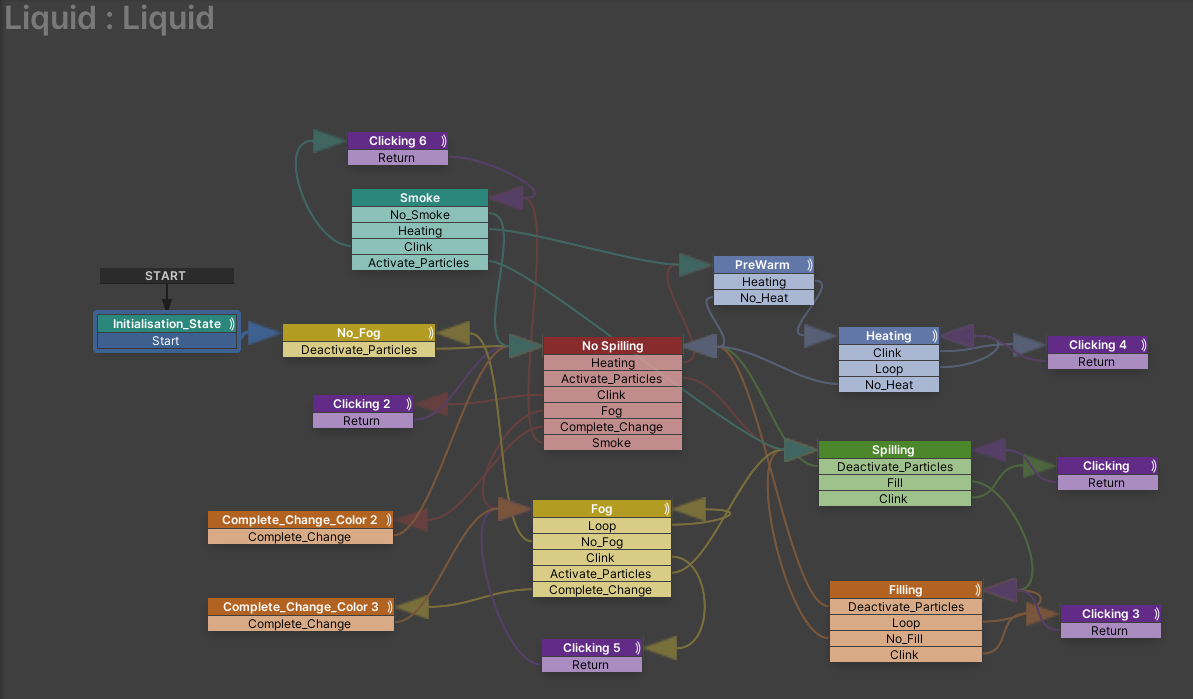
\includegraphics[width=0.7\textwidth, height = 7cm]{img/chapter05/Liquids.png}
    \caption{FSM Comportamiento de Liquidos}
    \label{fig:FSM_Liquids}
\end{figure}
\begin{itemize}
    \item Calentar líquidos: Al colocar un recipiente en un trípode con rejilla por encima de un mechero encendido, el líquido comienza a calentarse de manera progresiva. Este proceso está acompañado de efectos visuales como burbujeo y generación de vapor, que simulan las propiedades físicas reales del calentamiento.
    
    El estado del calentamiento se gestiona mediante la FSM correspondiente, que controla las transiciones entre los estados como ``Heating'' o ``PreWarm", dependiendo de la proximidad del recipiente al mechero y el tiempo de exposición al calor (ver \autoref{fig:FSM_Liquids}).
    \item Transferencia de líquidos entre recipientes: Los usuarios pueden verter líquidos de un recipiente a otro inclinando el primero, lo que activa estados como ``Spilling'' o ``Filling''. Estas acciones generan efectos visuales de derrame y llenado, junto con la actualización dinámica del nivel del líquido en ambos recipientes.
    \item Agregar sólidos a líquidos: La adición de polvos o sólidos genera reacciones químicas específicas, con cambios visuales como efervescencia o cambios de color, dependiendo del experimento.
\end{itemize}
\begin{figure}[thbp]
    \centering
    \begin{subfigure}[b]{0.3\linewidth}
        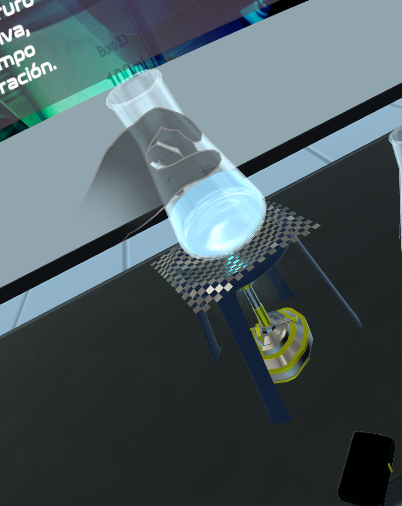
\includegraphics[width=\linewidth, height = 4cm]{img/chapter05/Calentamiento.png}
        \caption{Calentamiento de Líquidos}
        \label{fig:Calentamiento}
    \end{subfigure}
    \begin{subfigure}[b]{0.3\linewidth}
        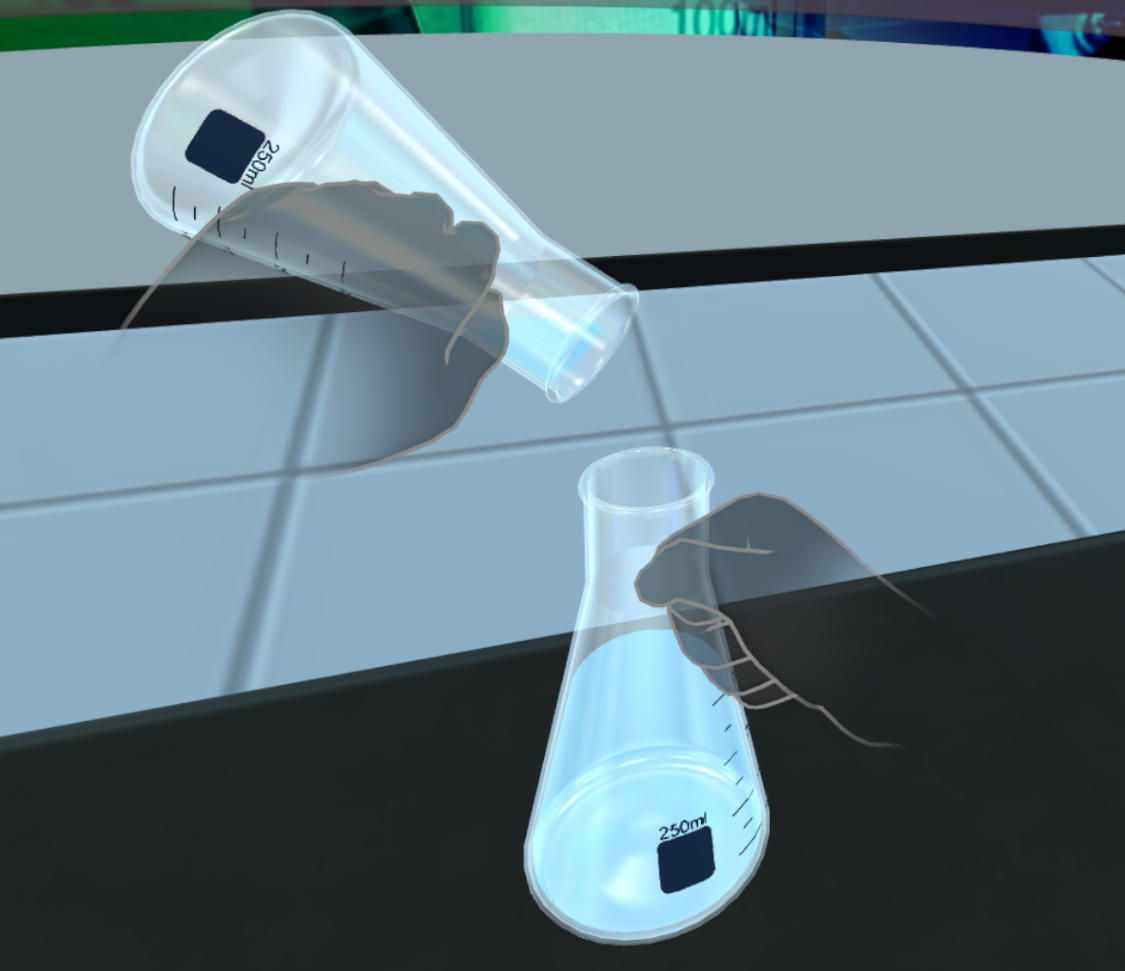
\includegraphics[width=\linewidth, height = 4cm]{img/chapter05/Vertido.png}
        \caption{Transferencia de Líquidos}
        \label{fig:Vertido}
    \end{subfigure}
    \begin{subfigure}[b]{0.3\linewidth}
        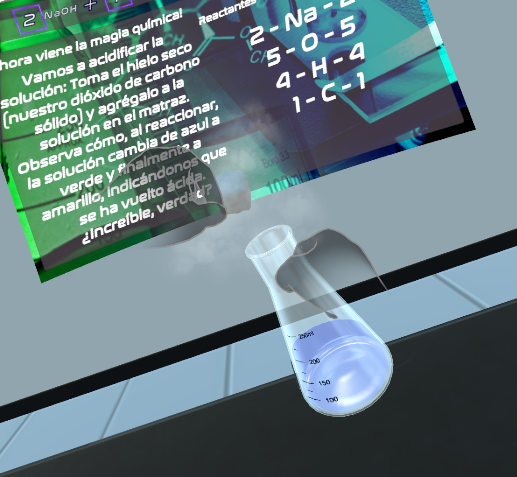
\includegraphics[width=\linewidth, height = 4cm]{img/chapter05/Agregar_Solidos.png}
        \caption{Interacción con Sólidos}
        \label{fig:Sólidos}
    \end{subfigure}
    \caption{Diversas Interacciones de Líquidos}
\end{figure}
